\documentclass{article}
\usepackage{amsmath}
\usepackage{amssymb}
\usepackage{graphicx}
\usepackage{hyperref}
\usepackage[version=4]{mhchem}

\title{Problem 17}
\date{}

\begin{document}
\maketitle

\section*{Problem}
Given \(\triangle A B C, \angle A=90^{\circ} . A B=A C . M\) is the midpoint of \(A C . A E \perp\) \(B M\) with the feet at \(E\). Extend \(A E\) to meet \(B C\) at \(D\). Prove that \(\angle A M B=\angle C M D\).\\
\centering
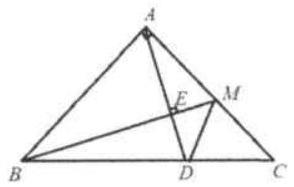
\includegraphics[width=\textwidth]{images/129(3).jpg}

\section*{Solution}
Draw \(C F / / A B\). Extend \(A D\) to meet \(C F\) at \(F\).\\
Since \(\angle A B M+\angle A M B=90^{\circ}\) and \(\angle M A E+\angle A M B=90^{\circ}\), \(\angle A B M=\angle C A F\).

Since \(A B=A C, \angle A B M=\angle C A F\). Rt \(\triangle A B M \cong\) Rt \(\triangle C A F\), \(\angle A M B=\angle F\).\\
\centering
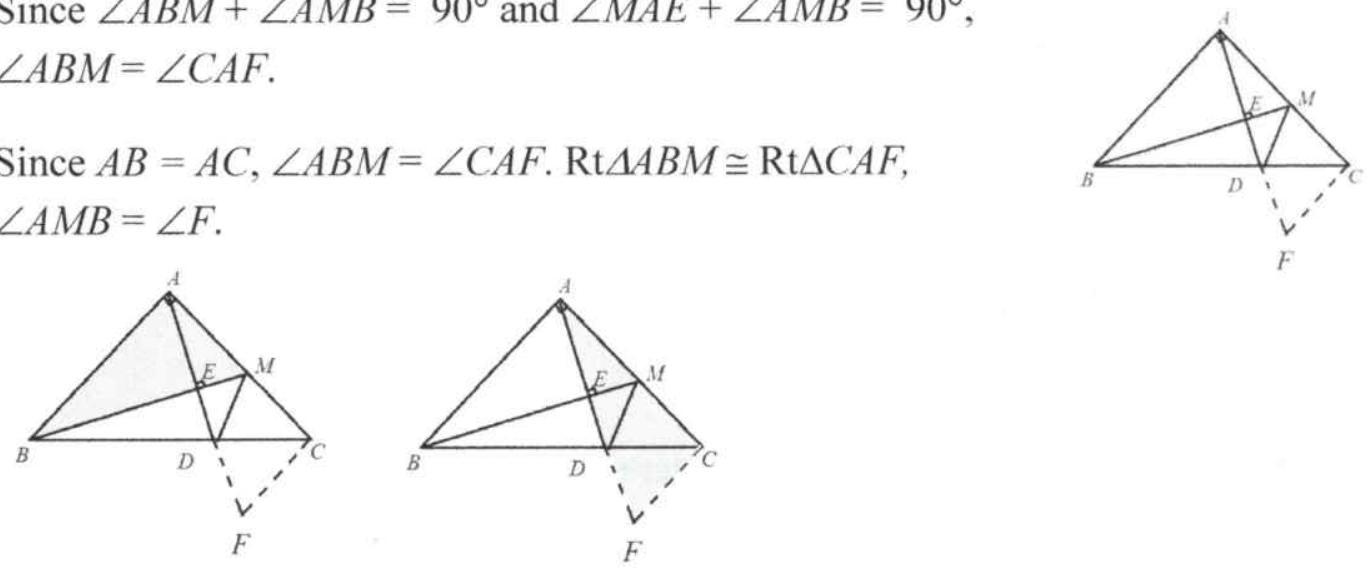
\includegraphics[width=\textwidth]{images/139(1).jpg}


Since \(\mathrm{MC}=\mathrm{AM}=\mathrm{CF}, \angle M C D=45^{\circ}=\angle F C D, \mathrm{CF}=\mathrm{CF}, \triangle M C D \cong \triangle F C D\).\\
\centering
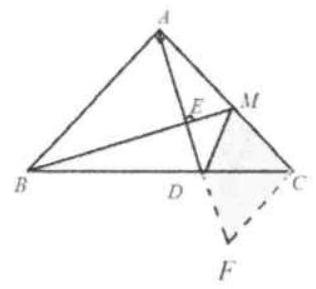
\includegraphics[width=\textwidth]{images/140(2).jpg}\\
\(\angle C M D=\angle F\).\\
Therefore, \(\angle A M B=\angle C M D\).

\end{document}
